\documentclass[activite]{thedocument}
\startdatakeys
\source{}
\BO{2026}
\cycle{4}
\competencesDuSocle{CH2,CA1}
\objectifsApprentissage{}
\motsCles{nombres premiers, crible d'Ératosthène, multiples}
\enddatakeys
\begin{document}
    \begin{center}
        \LARGE Crible d'ératostène
    \end{center}
    \vskip20pt
    L'objectif est de trouver rapidement tous les nombres premiers inférieurs à 100.
    \vskip20pt
    {\centering
    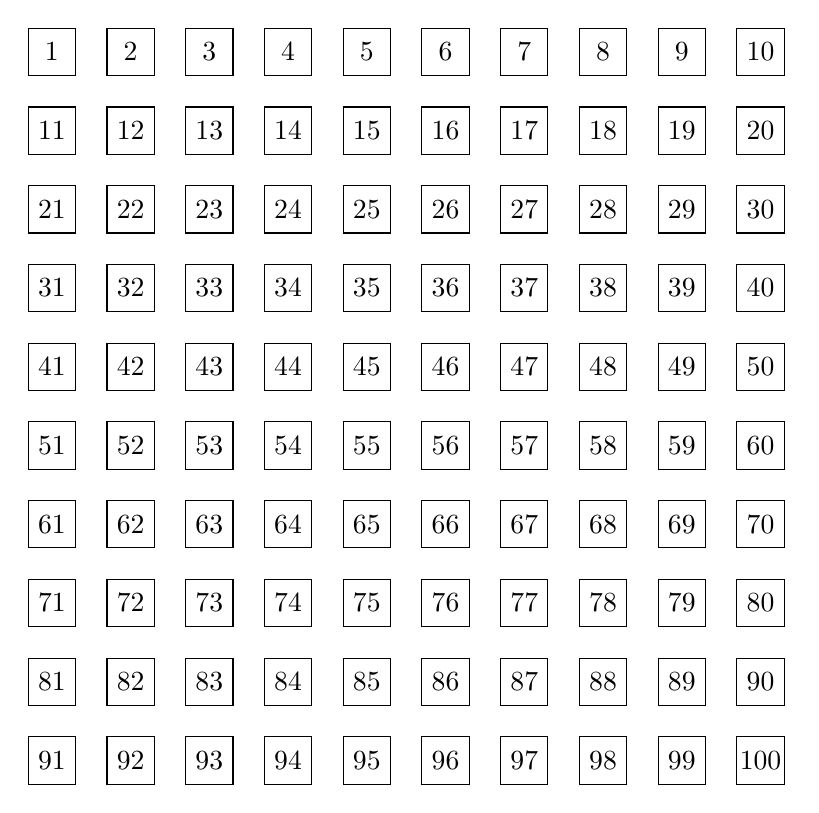
\begin{tikzpicture}
        \def\rectanglesize{0.3}
        \foreach\i in{0,1,...,9}{
            \foreach\j in{1,2,...,10}{
                \draw (\j-\rectanglesize,-\i-\rectanglesize)rectangle(\j+\rectanglesize,-\i+\rectanglesize);
                \draw node at(\j,-\i){\number\numexpr10*\i+\j};
            }
        }
    \end{tikzpicture}\par}
\end{document}